\documentclass[12pt]{article}
\usepackage{amsmath, amssymb, amsfonts}
\usepackage[margin=1in]{geometry}
\usepackage{setspace}
\usepackage{parskip}
\usepackage{fancyhdr}
\usepackage{graphicx}
\usepackage{subcaption}
\usepackage{color}
\usepackage{tikz}
\usetikzlibrary{shapes.geometric}
\usetikzlibrary{arrows.meta,arrows}

\pagenumbering{arabic}
\linespread{1.5}
\setlength{\parskip}{12pt}
\pagestyle{fancy}
\fancyhf{}

\lhead{Ningrui Xie}
\chead{BIO 4C12}
\rhead{ID: 400323416}
\fancyfoot[C]{\thepage}
\renewcommand{\headrulewidth}{0pt}

\newcommand{\perday}{\ensuremath{\mathrm{/day}}}
\newcommand{\Eqnref}[1]{Eq~\ref{#1}}
\newcommand{\eqnref}[1]{Eq~\ref{#1}}
\newcommand{\sref}[1]{Section~\ref{#1}}

\newcommand{\comment}{\showcomment}
%% \newcommand{\comment}{\nocomment}

\newcommand{\showcomment}[3]{\textcolor{#1}{\textbf{[#2: }\textsl{#3}\textbf{]}}}
\newcommand{\nocomment}[3]{}

\newcommand{\jd}[1]{\comment{cyan}{JD}{#1}}

\begin{document}

\title{Mathematical Approaches for Simulating Epidemic Progression: Addressing Limitations of the Linear Chain Trick in ODE Models}

\author{Submitted to\\ Dr. Jonathan Dushoff 
\\McMaster University\\Hamiltion, Ontario, Canada L8S 4K1}
\date {April 23, 2024}
\maketitle


\centerline{Reported by}
\centerline{\textbf{Ningrui Xie}}
\centerline{\textbf{400323416}}


\newpage
\section*{Abstract}
Simple dynamical models based on Ordinary Differential Equations (ODE) are widely utilized to forecast the spread of infectious diseases and to analyze other biological systems. A limitation of this framework is its implicit assumption that residence time in any given state, such as the infectious state, follows an exponentially distributed pattern. This assumption is often not realistic. A common solution is the application of the Linear Chain Trick (LCT), wherein a single stage is subdivided into multiple substages, each of which follows an identical exponential distribution, thereby yielding a more realistic Erlang distribution for the duration. However, the LCT poses challenges by restricting parametric flexibility, particularly resulting in less flexible dwell-time distributions, and it often necessitates comparisons between models with varying structures (i.e. different numbers of substages). Here, we propose a Geometric Chain Trick (GCT) employing a fixed number of substages with transition rates forming a geometric sequence. Through mathematical analysis, simulation, and model fitting, we demonstrate that our approach retains the principal benefits of the LCT while providing increased flexibility and facilitating easier data fitting. Compared to the recently introduced Generalized Linear Chain Trick (GLCT), which incorporates higher-dimensional auxiliary stages to model delays in transitions between main compartments, our method offers a more direct means of achieving flexibility. Although this study focuses on the application of the LCT and GCT in the epidemic SIR (susceptible-infectious-recovered) model, the potential applications of our approach span a broad array of dynamical models, including those for infectious diseases and other systems (e.g. population dynamics, biochemical reaction networks), offering advantages in computational efficiency, ease of parameter estimation, and the flexibility of time distributions.

\section{Introduction}
Ordinary differential equations (ODEs) are extensively utilized for mathematical modeling in the biological sciences, offering a robust framework to describe the temporal dynamics of systems. Their capacity to model continuous state changes makes them essential in capturing complex biological phenomena such as population dynamics \cite{salisbury2011mathematical}\cite{sego2021generation}, epidemiological patterns of infectious diseases \cite{Anderson1991}\cite{Diekmann2000}\cite{Feng2016}, and cellular processes like proliferation in oncogenesis \cite{baker1998modelling}\cite{jarrett2018mathematical}. The inherent flexibility and simplicity of ODEs make them not only easy to solve and understand but also easy to manipulate and accommodate to various situations.

In the field of epidemiology, ordinary differential equations (ODEs) serve as a crucial tool for characterizing disease progression and making predictions. During the COVID-19 pandemic, they were extensively utilized to guide policy-making, especially in disease control and public health interventions \cite{thompson2020epidemiological}. A commonly used model is the SIR compartmental model \cite{Anderson1991}\cite{kermack1927contribution}, which divides the population into three states: Susceptible $(S)$, Infectious $(I)$, and Recovered $(R)$. In the model, a susceptible individual, upon contact with the infected population at a rate $\beta$ $[\frac{1}{\mathit{ time}}]$, transitions immediately to the infectious state. An infected individual then moves to the recovered state at a recovery rate of $\gamma$ $[\frac{1}{\mathit{time}}]$. A major limitation of this model is its implicit assumption that the duration of the infectious stage follows an exponential distribution. This can be observed in a simplified equation that models the dynamics of an infected cohort. The proportion of a cohort infected at the same time begins at 1, and follows:
\begin{align}
    \frac{dI}{dt} = -\gamma I
\end{align}
Solving this equation explicitly yields
\begin{align}
    I(t) = e^{-\gamma t}.
	 \label{explicitCohort}
\end{align}
In other words, the time spent in the infectious stage $I$ is exponentially distributed with a mean stage duration of $\frac{1}{\gamma}$.
\Eqnref{explicitCohort} implies that an individual has the highest probability of recovering from the disease immediately after infection, which is generally not realistic. In reality, a delay between the successful infection of an individual and the recovery from the disease is inevitable. The work conducted by Byrne AW et al.~\cite{byrne2020inferred} presents the simulation of parameter distribution inferred for the duration of the infectious period, and the shape of this distribution closely resembles a gamma distribution.

Even when the mean is constant, the shape of the stage duration distributions (i.e., the timing of stage transitions) can significantly impact the dynamics and the outcomes of predictive models in applied settings \cite{krylova2013effects}\cite{keeling2002understanding}\cite{wearing2005appropriate}\cite{nguyen2008noise}. Consequently, it becomes crucial to consider the type of distribution characterizing an individual in a specific state when constructing these models. A standard approach for developing models that incorporate different stage duration distributions is through the use of integro-differential equations (IDEs) or integral equations (IEs) \cite{hurtado2019generalizations}\cite{kermack1927contribution}\cite{hethcote1980integral}. IDEs facilitate the extension of the SIR model to include arbitrary distributions for the duration of infectiousness, as discussed in various sources \cite{feng2000endemic}\cite{hethcote1980integral}\cite{ma2006generality}. This approach allows for the capture of the `memory effect', where the current rate of change in each compartment of the model (Susceptible, Infectious, Recovered) is influenced by the entire history of the epidemic, rather than relying on a constant rate assumption.

However, while integro-differential equations increase the model's flexibility, they present challenges in formulation, mathematical analysis, and simulation, particularly in comparison to ODEs \cite{krylova2013effects}\cite{hurtado2019generalizations}\cite{burton2005volterra}. An alternative method, the Linear Chain Trick (LCT), overcomes some of these challenges, offering a simpler and more direct approach to modifying the shape of distributions \cite{macdonald1978time}\cite{smith2011introduction}. This approach subdivides the single infected state into n substages, each characterized by an identical exponential distribution with a rate of $n\gamma$. This technique is based on the principle that the sum of a series of independent exponentially distributed random variables follows an Erlang distribution \cite{krylova2013effects}\cite{therrien2018probability}, which is a special case of the gamma distribution with an integer shape parameter. By employing this method, the distribution of the infectious stage duration transitions from exponential to Erlang. The central tendency of the Erlang distribution towards its mean value offers the model a more accurate representation of real-world scenarios.

When applying LCT into the SIR model, the number of substages $n$ determines the shape of the stage duration distribution. As $n$ increases, the variance decreases, resulting in a distribution that is more peaked and narrow. As $n$ approaches infinity, the distribution converges to a delta function (a deterministic value, implying that all individuals who become infectious at time $t$ recover at exactly time $t + \frac{1}{\gamma}$), and the system approaches a delay differential equation \cite{krylova2013effects}\cite{hethcote1980integral}.

The Linear Chain Trick (LCT) is extensively employed in modeling biological processes, not only in quantifying disease progression \cite{lloyd2001destabilization}\cite{lloyd2001realistic}, but also in analyzing virus \cite{lloyd2001dependence}\cite{kakizoe2015method} and population \cite{cushing2013integrodifferential} dynamics. Studies have demonstrated that switching the stage duration distribution from an exponential to an Erlang distribution leads to predictions that align more closely with real data points \cite{kakizoe2015method}. But employing LCT in ODE models presents important limitations. First is inflexibility: the number of substages, $n$, must be an integer. Another limitation is the cumbersome and time-consuming process of determining the appropriate number of substages to use. Multiple models with varying substages must be constructed and fitted to identify the optimized parameter value. Prior research has investigated approaches for estimating the number of states in the linear chain, employing techniques such as profile likelihood \cite{raue2009structural} and model reduction \cite{maiwald2016driving}. A comparative study of these methods indicates that the typical quality of experimental data is insufficient for reliably estimating the chain length using these approaches \cite{hauber2020estimating}. These limitations significantly restrict the adaptability and practical application performance of the model.

The recently proposed Generalized Linear Chain Trick (GLCT) enhances the Linear Chain Trick (LCT) by enabling models to incorporate a broader phase-type family of distributions \cite{hurtado2019generalizations}\cite{hurtado2021building}\cite{bladt2017phase}, which includes exponential, Erlang, hypoexponential, and Coxian distributions, thus allowing for greater flexibility and the ability to capture more complexity. The GLCT achieves this by creating a higher-dimensional Markov chain, enabling a more accurate representation of the complex nature of dwell time distributions. However, this process can be mathematically heavy and challenging to interpret. Additionally, this approach may lead to a increase in the number of variables or states within the model, potentially escalating computational demands. Therefore, finding a simpler and more efficient method to enhance the flexibility of the ODE model remains essential.

In this study, we focused on one particular direction: generalizing the Erlang distribution of stage durations currently present in the model. The goals were to have a more effective way for parameter estimation and to eliminate the constraints imposed on the shape parameter ($\kappa$). To address these limitations, we proposed the Geometric Chain Trick (GCT). Instead of having a variable number of substages $(n)$ with a constant transition rate between them $(\gamma_i = n\gamma)$, we fix $n$ to a specific integer value and use a series of rates that follow a geometric pattern. This series is represented by the formula $\gamma_i = ar^{i-1}$, governed by parameters $a$ and $r$. This approach enables a uniform model structure with the parameter of interest transitioning from discrete values $(n$ and $n\gamma)$ to continuous values $(a$ and $r)$, thereby enhancing the model's adaptability (details in \sref{Models}).

To illustrate this point, consider that the Gamma distribution can be parameterized in terms of its mean $(D)$ and shape parameter (quadratic coefficient of variation, $\kappa$), which determine the overall shape and position of the distribution. As mentioned above, in subdividing a single stage into n substages, each exponentially distributed substage must have a rate of $n\gamma$ to maintain the overall rate of that stage. While the mean of the Erlang distribution in the ODE system can be chosen freely, $\kappa$ is constrained to discrete values, shown as follows:
\begin{align*}
    Mean: \quad &\sum_{i=1}^{n_f} \frac{1}{n\gamma} = \frac{1}{\gamma}\\
    Variance: \quad &\sum_{i=1}^{n_f} \frac{1}{n^2\gamma^2} = \frac{1}{n\gamma^2} \\
    \kappa: \quad &\frac{\sigma^2}{M^2} = \frac{1}{n} \quad n \in \mathbb{N}
\end{align*}
Our approach, using a geometric series of rates, addresses this issue by allowing $\kappa$ to take any value within the range $\left[ \frac{1}{n}, 1 \right)$. A detailed explanation and the derivation process are provided in \sref{parm result}. Another advantage of this method is that it enables a fixed model structure where only the parameters change, eliminating the need to determine optimal substage numbers through the construction of multiple models, a process currently required in the ODE model that employs the LCT.

Throughout this research, we primarily focused on the application of the LCT in the epidemic SIR model, which we refer to as the LCT model (or SI$^n$R model, where $n$ represents the number of substages divided). The objective of our study is to develop and evaluate the method of using a fixed model structure and a geometrically distributed substage rate as a replacement for the constant rate, aiming to enhance flexibility and efficiency. We have named the model that utilizes this method the GCT model. We anticipate that this approach will not only be computationally efficient but also provide a better fit to real-world data. In the following sections, we first analyze the model parameters by calculating the formulae for two essential properties: the mean and shape parameter. We then invert the process: given a desired $D$ and $\kappa$, we develop a computational system to determine the parameter values $a$ and $r$ that enable the model to produce a stage duration distribution with these properties. The obtained parameter values are then used to compare the GCT model with the LCT model through simulation. Subsequently, we conduct empirical validation of our model through data fitting. This fitting confirmed that the GCT model enables the use of a uniform model structure with enhanced flexibility and practicality, thus paving the way for the development of user-friendly software tools that empower modelers to efficiently select and employ the most suitable models for describing and predicting future epidemic scenarios.


\section{Models}
\label{Models}
Several assumptions have been made for the unforced SIR model (Susceptible, Infectious, and Recovered) that our study is based on: 
\begin{enumerate}
    \item \textbf{Closed Population}: A constant population size with equal birth and death rates and no disease-related mortalities.
    \item \textbf{Homogeneous mixing}: Individuals have an equal chance of coming into contact with any other individual in the population. 
    \item \textbf{Ignoring Latency}: Individuals move immediately from a susceptible state to an infected state, ignoring any incubation period associated with the disease.
    \item \textbf{Lifelong immunity}: Once an individual recovers, they do not become susceptible or infectious again.
    \item \textbf{Fixed rate of transmission and recovery}: The rate of disease spread and the rate at which infected individuals recover and become immune are constant over time.
\end{enumerate}

The dynamic of the population within the three compartment can be expressed as a system of nonlinear ordinary differential equations:
\begin{align}
    \frac{dS}{dt} &= \mu N - \frac{\beta SI}{N} - \mu S \\
    \frac{dI}{dt} &= \frac{\beta SI}{N} - \gamma I - \mu I \\
    \frac{dR}{dt} &= \gamma I - \mu R
\end{align}
where $S$, $I$, and $R$ represent the susceptible, recovered, and infectious population. $N$ is the size of the total population, and in this case $S + I + R = N$. $\mu$, $\beta$ and $\gamma$ are the rates of natural birth (death), transmission, and recovery, respectively. $\beta$ is the rate of new infections per unit time, so $\frac{\beta SI}{N}$ is the number of new infections that occur per unit time (the incidence rate). Together, formulas $(3,4,5)$ will be referred to as the transmission model. Here, the mean recovery time for an infected individual is $\frac{1}{\gamma}$. By assuming that the entire population was infected at the onset and considering a zero natural birth (death) rate, we can focus solely on the dynamics of the recovered population, as indicated by formula (1). 

The idea of dividing the infectious stage into $n$ sub-stages exploits the fact that the sum of a sequence of independent, exponentially distributed random variables follows an Erlang distribution (i.e. gamma distributed with integer shape parameter) \cite{therrien2018probability}
\begin{equation}
    f(x; n,n\gamma) = \frac{(n\gamma)^n}{(n-1)!} x^{n-1} e^{-n\gamma x} \quad x>0, n \in \mathbb{N}
\end{equation}
Utilizing the principle of the Linear Chain Trick (LCT), we divide the single infectious stage into $n$ substages, each with a constant rate of $n\gamma$ (Figure \ref{LCTdiagram}). 
\begin{figure}[ht]
    \centering
    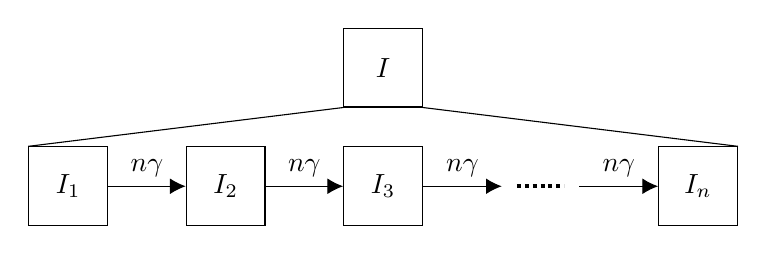
\begin{tikzpicture}[scale=1, transform shape, >={Latex[length=2mm, width=2mm]}]
        \node (I) at (0,1) [draw, minimum width=1cm, minimum height=1cm] {$I$};
        
        % Nodes I1 to In
        \node at (-4,0) [below, draw, minimum width=1cm, minimum height=1cm] (I1) {$I_1$};
        \node at (-2,0) [below, draw, minimum width=1cm, minimum height=1cm] (I2) {$I_2$};
        \node at (0,0) [below, draw, minimum width=1cm, minimum height=1cm] (I3) {$I_3$};
        \node at (4,0) [below, draw, minimum width=1cm, minimum height=1cm] (In) {$I_n$};
        
        % Dots
        \draw[line width=0.5mm, dotted, dash pattern=on 0.5mm off 0.5mm] (1.7,-0.5) -- (2.3,-0.5);
        
        % Arrows
        \draw[->] (I1.east) -- (I2.west) node[midway, above] {$n\gamma$};
        \draw[->] (I2.east) -- (I3.west) node[midway, above] {$n\gamma$};
        \draw[->] (I3.east) -- ([xshift=1cm]I3.east) node[midway, above] {$n\gamma$};
        \draw[->] ([xshift=-1cm]In.west) -- (In.west) node[midway, above] {$n\gamma$};
        
        %\draw[-latex] (In.east) -- ([xshift=2cm]In.west) node[midway, above] {$n\gamma$};
        
        % Arrows from I to I1 and In
        \draw[-] (I.south west) -- (I1.north west);
        \draw[-] (I.south east) -- (In.north east);

    \end{tikzpicture}
    \caption{Example diagram of the Linear Chain Trick}
    \label{LCTdiagram}
\end{figure}

Therefore, formula (1) will be replaced by the following set of equations (7-10), which we refer to as the cohort model:
\begin{align}
    \frac{dI_1}{dt} &= - n \gamma I_1 \\
    \frac{dI_2}{dt} &= n\gamma I_1 - n \gamma I_2 \\
    &\vdots \\
    \frac{dI_n}{dt} &= n\gamma I_{n-1} - n \gamma I_n \\
    \frac{dR}{dt} &= n \gamma I_n
\end{align}
Note that this decomposition process will not change the mean stage duration, as the sum of the means of the $n$ exponentially distributed random variables still equals $\frac{1}{\gamma}$
\begin{align*}
    \sum_{i=1}^{n} \frac{1}{n\gamma} = \frac{1}{\gamma}
\end{align*}

The Geometric Chain Trick (GCT), on the other hand, features a fixed number of substages along with a set of inter-substage transition rates characterized by a geometric series $\gamma_i = ar^{i-1}$ (Figure \ref{GCTdiagram}), rather than a constant rate, as illustrated below (12-16):
\begin{align}
    \frac{dI_1}{dt} &= - a I_1 \\
    \frac{dI_2}{dt} &= a I_1 - ar I_2 \\
    \frac{dI_3}{dt} &= ar I_2 - ar^2 I_3 \\
    &\vdots \\
    \frac{dI_n}{dt} &= ar^{n-2} I_{n-1} - ar^{n-1} I_n \\
    \frac{dR}{dt} &= ar^{n-1} I_n
\end{align}

\begin{figure}[ht]
    \centering
    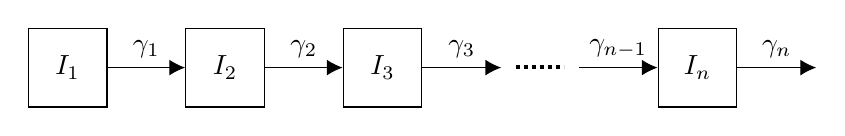
\begin{tikzpicture}[scale=1, transform shape, >={Latex[length=2mm, width=2mm]}]
        
        % Nodes I1 to In
        \node at (-4,0) [below, draw, minimum width=1cm, minimum height=1cm] (I1) {$I_1$};
        \node at (-2,0) [below, draw, minimum width=1cm, minimum height=1cm] (I2) {$I_2$};
        \node at (0,0) [below, draw, minimum width=1cm, minimum height=1cm] (I3) {$I_3$};
        \node at (4,0) [below, draw, minimum width=1cm, minimum height=1cm] (In) {$I_n$};
        
        % Dots
        \draw[line width=0.5mm, dotted, dash pattern=on 0.5mm off 0.5mm] (1.7,-0.5) -- (2.3,-0.5);
        
        % Arrows
        \draw[->] (I1.east) -- (I2.west) node[midway, above] {$\gamma_1$};
        \draw[->] (I2.east) -- (I3.west) node[midway, above] {$\gamma_2$};
        \draw[->] (I3.east) -- ([xshift=1cm]I3.east) node[midway, above] {$\gamma_3$};
        \draw[->] ([xshift=-1cm]In.west) -- (In.west) node[midway, above] {$\gamma_{n-1}$};
        \draw[->] (In.east) -- ([xshift=1cm]In.east) node[midway, above] {$\gamma_n$};
        
        %\draw[-latex] (In.east) -- ([xshift=2cm]In.west) node[midway, above] {$n\gamma$};
    

    \end{tikzpicture}
    \caption{Example diagram of the Geometric Chain Trick}
    \label{GCTdiagram}
\end{figure}

Having established the model, our initial step involved analyzing the parameters within the GCT model. We aim to determine whether employing a fixed model structure (i.e., a fixed number of substages) and manipulating the parameters $a$ and $r$, which define the geometric transition rate, can achieve the same effects as varying the number of substages. Additionally, we aim to evaluate whether the GCT structure offers greater flexibility in the choice of $\kappa$ $(CV^2)$. By calculating the mean $(D)$, variance $(\sigma)$, and shape parameter $(\kappa)$, we are able to represent all these properties of the infectious stage duration distribution in terms of $a$ and $r$. Similar to the LCT, utilizing the GCT facilitates independent alterations in the mean and $\kappa$. Given this, we can invert the process: starting with specific values of $D$ and $\kappa$, we can identify the corresponding $a$ and $r$ that endow the model with such characteristics. However, due to the complexity of the formula, solving it explicitly is challenging. To overcome this, we have developed a system of functions in the \textbf{R} programming language, employing \verb|uniroot()| to determine the values of $a$ and $r$. These parameters are then integrated to the GCT model to compare simulation outcomes with those of the LCT model, examining alignment in both the infectious stage duration distribution and the incidence over time.

After confirming that the GCT model, which employs a fixed structure and varying parameters $a$ and $r$, achieves comparable efficacy to the LCT model, we proceeded to empirically test the model's enhanced performance. Specifically, we focused on its improved flexibility in the kappa parameter through data fitting. Initially, we utilized simulated data as a replacement for actual data. This incidence data was generated through transmission model simulations, with deviations (noise) introduced via a mean reporting ratio and a negative binomial dispersion parameter. We performed model fitting using the \textbf{bbmle} package in R, estimating the model parameters through Maximum Likelihood Estimation (MLE). Our goal was to accurately retrieve the parameter values used to generate the incidence data, assessing the fitting quality through the root mean squared log error (RMSLE).

We began by applying the same model type (LCT or GCT) for both data generation and model fitting. Data were generated by simulating the LCT model with two substages $(n=2)$ and then fitted using the LCT model, evaluating both identical and modified structures. This methodology was similarly applied to the GCT model. To further test the GCT model, we increased the fitting challenge by generating incidence data using the LCT model and then fitting it with the GCT model, varying the number of substages. Subsequently, we modified both the fitting model's structure and the input data to observe the impact on fitting outcomes. Finally, we extracted the parameters estimated through fitting and compared them with the actual values (those used for simulation).

In the next phase of our study, we will approach the fitting of interval data from two perspectives: the rounding paradigm, which interprets 2 days as meaning any duration between 1.5 and 2.5 days, and the start/end paradigm, which considers potential starting and ending times. Initially, we will generate interval data using various distributions, such as gamma and lognormal, and subsequently apply both the LCT and GCT models for fitting. Although the GCT model can replicate certain properties (such as $D$ and $\kappa$) observed with the gamma distribution, its inherent distribution does not match the gamma distribution precisely. Thus, it's necessary for us to develop a new likelihood function for fitting purposes. Furthermore, we intend to incorporate real-world data, including incidence and interval data, to evaluate the GCT model's performance comprehensively. By comparing the fitting results from both the LCT and GCT models, we aim to quantitatively determine the effectiveness of our proposed method in enhancing model accuracy and its reflection of actual epidemiological scenarios.

\section{Results}
\subsection{Independent and Flexible Modification of Mean and Kappa in Stage Duration Distribution Using the GCT Model}
\label{parm result}
As discussed in previous sections, the duration distribution of the stage can be parameterized by its mean (D) and shape parameter $(\kappa^2 = CV^2)$. In the GCT model, the calculation of mean and variance is achieved by summing the respective properties of each substage, shown as follows:
\begin{align}
    Mean: \quad  &\sum_{i=1}^{n_f} \frac{1}{\gamma_i} = \frac{\frac{1}{a} (\frac{1}{r^n} - 1)}{\frac{1}{r} -1} \\
    Variance: \quad &\sum_{i=1}^{n_f} \left(\frac{1}{\gamma_i} \right)^2 = \frac{\frac{1}{a^2} (\frac{1}{r^{2n}} - 1)}{\frac{1}{r^2} -1}
\end{align}
The shape parameter $\kappa$, determined by $\frac{\sigma^2}{D}$, can thus be obtained:
\begin{align}
    \kappa = \frac{(1+r^{n}) (1-r)}{(1+r) (1-r^{n})}
\end{align}
This simplification revealed that the value of $\kappa$ is solely determined by the parameter $r$, thus enabling the alignment of kappa without affecting the mean, which can be adjusted through alterations to parameter $a$. Similarly, the mean can be scaled to a desired value without impacting $\kappa$. This grants the model independence in modifying properties.

Importantly, within the GCT model, the value of $\kappa$ becomes independent of this number. It should also be noted that, according to formula (20), the range of $\kappa$ can encompass any real number within the range $\left[ \frac{1}{n}, 1 \right)$ for $r > 0$, thereby enhancing the model's flexibility. In contrast, when applying a similar calculation for $\kappa$ in the LCT model, we find that $\kappa = \frac{1}{n}$ and the shape parameter is therefore constrained to a series of discrete values, as follows:
\begin{align*}
    \kappa \in \left\{ 1, \frac{1}{2}, \frac{1}{3}, \dots \right\}
\end{align*}
The transition from discrete to continuous values in kappa increases the model's adaptability to the shape of the stage duration distribution, enabling a more precise fit to the observed data and allowing for a nuanced interpretation of temporal patterns.

\subsection{Matching GCT and LCT Model Performance through Parameter Adjustment within a Uniform Structure}

Using formulas (18) and (20), we developed code to reverse-engineer the process: given specific values of D and kappa, we can identify the corresponding $a$ and $r$ that endow the model with such characteristics. These $a$ and $r$ values were subsequently integrated into the GCT model. Our initial goal was to determine if the stage duration distribution could match between the two models, assuming identical $D$ and $\kappa$ values. The number of substages in the LCT model was set to 2, 4, 6, and 8, while the substage number for the GCT model was fixed at 12. We selected a mean of 10 days. Applying the mean and kappa values $\left[ \frac{1}{2}, \frac{1}{4}, \frac{1}{6}, \frac{1}{8} \right]$ to the system, we plotted the stage duration distributions generated from the LCT cohort model alongside those from the GCT with the corresponding a and r values. As depicted in Figure \ref{distributionCompare}, the stage duration distributions exhibit slightly different shapes, despite having identical mean and shape parameters. To further examine the match of properties, D and kappa were numerically calculated from the output distributions, revealing identical values across both models. This indicates that while the distributions' shapes may not completely match, they can possess the same properties.

\begin{figure}[h!]
    \centering
    \includegraphics[width=\textwidth]{figures/distributionCompare.Rout.pdf}
    \caption{\textbf{Stage Duration distribution Comparsion between LCT and GCT.} \\ Duration of the infectious stage derived from the derivative of infectious population dynamics in simulations of the GCT (Geometric Chain Trick) and LCT (Linear Chain Trick) cohort models, with a mean infectious recovery period of 10 days $(\gamma = \frac{1}{10})$. The GCT model features a fixed substage number of 12, whereas the LCT model's substage number varies and is indicated in each figure's title. $\kappa$ values are calculated as $\frac{1}{n}$ for each plot. Parameters for the GCT model were adjusted to standardize the mean $(D)$ and shape parameter $(\kappa)$ across all distributions.}
    \label{distributionCompare}
\end{figure}


By reintegrating the infectious stage duration distribution into the whole dynamic system, we present the dynamics of newly infected cases (incidence) as simulated by the transmission model. Figure \ref{incidenceCompare} illustrates the incidence time series for the LCT model with 4 and 8 substages, represented by yellow and blue lines, respectively. The corresponding kappa values of the stage duration distribution for them are $\frac{1}{4}$ and $\frac{1}{8}$. All other parameters are held constant. All other parameters are identical across the two models. Employing the GCT model with a fixed 12 substages and utilizing $a$ and $r$ values derived from the reverse-engineering system for the targeted kappa values, we successfully approximate the incidence patterns observed in the LCT model across different substage configurations, as shown by the black dashed line. This demonstrates the GCT model's capability to match the LCT model's performance by adjusting parameters within a constant structural framework. Compared to modifying the model structure to achieve desired kappa values, the GCT model simplifies parameter estimation and model fitting processes. 

\begin{figure}[h!]
    \centering
    \includegraphics[width=\textwidth]{figures/incidenceCompare.Rout.pdf}
    \caption{\textbf{Incidence comparsion between GCT and LCT with different substage numbers} \\ Incidence over time for GCT and LCT transmission models, depicted under a mean recovery period of 10 days $(\gamma = \frac{1}{10})$, with $\beta=0.2$, $\mu=0.001$, $N=1$, $I_0=0.01$. The incidence from the LCT model is illustrated with a blue line for 4 substages and a yellow line for 8 substages. The black dashed line represents the GCT model incidence, featuring a uniform 12 substages, with adjusted $a$ and $r$ values to align the $\kappa$ value with that of the LCT model. This ensures both models have comparable $D$ and $\kappa$ values across the depicted incidences.}
    \label{incidenceCompare}
\end{figure}


\subsection{Substage Configuration Minimally Impacts Model Fitting}

After establishing the theoretical foundation, we proceeded with model fitting to assess the GCT model's performance. The incidence data were obtained from the model simulation, and the noises were added using a mean reporting ratio of 0.9 and a negative binomial dispersion parameter of 1000. Initially, we employed the same model type for both data generation and fitting. In Figure \ref{sametypeFittingL}.A, the data, generated by the LCT model with 2 substages, were fitted using an LCT model of the identical structure, as the plot title indicates. The quality of the fitting was evaluated based on the root mean squared logarithmic error (RMSLE), which measured the percentage errors between the actual and predicted value. With an RMSLE value of 1.64\%, the fitting can be considered satisfactory. Figure \ref{sametypeFittingL}.B showcases the parameters estimated post-fitting along with their 95\% confidence intervals, with the target value represented by the red line. Conversely, employing the same incidence data but altering the fitting model's structure from an LCT with 2 substages to an LCT with 6 substages, as depicted in Figure \ref{sametypeFittingL}.C, resulted in less favorable outcomes, with the RMSLE escalating to 9.30\%. The estimated parameters, displayed in Figure \ref{sametypeFittingL}.D, showed significant discrepancies. 

\begin{figure}[h!]
    \centering
    \begin{tikzpicture}
        \node[anchor=south west,inner sep=0] (image) at (0,0) {\includegraphics[width= \textwidth]{figures/sametypeFittingL.Rout.pdf}};
        \begin{scope}[x={(image.south east)},y={(image.north west)}]
            % Add labels at desired positions
            \node at (0.01,0.95) {\textbf{(A)}};
            \node at (0.55,0.95) {\textbf{(B)}};
            \node at (0.01,0.45) {\textbf{(C)}};
            \node at (0.55,0.45) {\textbf{(D)}};
        \end{scope}
    \end{tikzpicture}
    \caption{\textbf{Model fitting and parameter estimation in LCT model.} \\ Data generated form the LCT transmission model featured 2 substages, with $\beta=0.2$, $\mu=0.01$, $N=10000$, $I_0=10$. The parameters fitted are $\beta$ and $D$. Plots A and C show the fitting results (red), alongside the target values (green) and the input data to the model, after adding noise (blue), using 2 and 6 substages, respectively. Plots B and D present the estimated parameters post-fitting. Each parameter's 95\% confidence interval is shown, with the exact values highlighted by a red line.}
    \label{sametypeFittingL}
\end{figure}

Not surprisingly, employing the GCT model with 12 substages for both generating and fitting incidence data also resulted in a close match, as indicated by an RMSLE of 2.34\% (Figure \ref{sametypeFittingG}.A), and parameters post-fitting were close to the exact values (Figure \ref{sametypeFittingG}.B). Unlike the case with the LCT model, when the structure of the fitting model was altered from 12 substages to 6, the model still exhibited a close match with the original in terms of both shape (Figure \ref{sametypeFittingG}.C) and parameters (Figure \ref{sametypeFittingG}.D). This indicates that the GCT model's fitting performance is minimally impacted by changes in the model structure.

\begin{figure}[h!]
    \centering
    \begin{tikzpicture}
        \node[anchor=south west,inner sep=0] (image) at (0,0) {\includegraphics[width= \textwidth]{figures/sametypeFittingG.Rout.pdf}};
        \begin{scope}[x={(image.south east)},y={(image.north west)}]
            % Add labels at desired positions
            \node at (0.01,0.95) {\textbf{(A)}};
            \node at (0.55,0.95) {\textbf{(B)}};
            \node at (0.01,0.45) {\textbf{(C)}};
            \node at (0.55,0.45) {\textbf{(D)}};
        \end{scope}
    \end{tikzpicture}
    \caption{\textbf{Model fitting and parameter estimation in GCT model.} \\ Data generated from the GCT model featured 2 substages, with kappa= $\beta=0.2$, $\mu=0.01$, $N=10000$, $I_0=10$ and $\kappa=\frac{2}{9}$. Remaining details are as described in Figure \ref{sametypeFittingL}.}
    \label{sametypeFittingG}
\end{figure}

%%%%%%%%
% Here
%%%%%%%%
To more clearly illustrate the performance differences between the LCT and GCT models, fittings with various model structures were conducted to assess changes in percentage error. The percentage error from the fitting result, where the model generating the incidence data and the model for fitting are exactly the same, has been used as the baseline (red line). As shown in Figure \ref{rmsle}, when using the same input data, varying the fitting model shape causes the LCT model to experience a surge in RMSLE values, while the GCT model maintains its error rate close to the baseline. This result, once again, confirms that the structure of the GCT model merely affects the fitting results, indicating that changes in structure to optimize model performance are no longer necessary.

\begin{figure}[h!]
    \centering
    \includegraphics[width=\textwidth]{figures/rmsle.Rout.pdf}
    \caption{\textbf{Percentage error with different fitting model structures.} \\ The LCT fitting data were generated by simulating a two-substage LCT transmission model with $D=10, \beta=0.2$, $\mu=0.01$, $N=10000$, $I_0=10$. Similarly, GCT fitting data came from simulating the GCT model with identical properties but $\kappa=\frac{5}{9}$. The baseline (red) represents the error rate when the fitting and data generation models have the same structure. The blue circle indicates LCT errors, and the orange rhombus represents GCT errors.}
    \label{rmsle}
\end{figure}


\subsection{Adaptability of the GCT Model to Data Input and Structural Changes in Fitting}
Proceeding to a more challenging test, we utilized a different model type for data generation and model fitting. As demonstrated in Figure \ref{difftypeFitting}.A, the data generated by the LCT model with 2 substages were fitted using the GCT model with 12 substages. Despite the significant difference in model structure, the fitting results were reasonably favorable, with an RMSLE of 2.44\%. Altering the fitting model from a GCT with 2 substages to a GCT with 6 substages had negligible impact on the fitting outcomes (Figure \ref{difftypeFitting}.B). Similarly, changing the input data from an LCT with 2 substages to an LCT with 7 substages resulted in slightly improved fitting, though the difference was not substantial (Figure \ref{difftypeFitting}.C). These findings suggest that regardless of changes to the fitting model structure or the data used, the GCT model is capable of adapting to these variations, providing satisfactory fitting results.

\begin{figure}[h]
    \centering
    \begin{tikzpicture}
        \node[anchor=south west,inner sep=0] (image) at (0,0) {\includegraphics[width= \textwidth]{figures/difftypeFitting.Rout.pdf}};
        \begin{scope}[x={(image.south east)},y={(image.north west)}]
            % Add labels at desired positions
            \node at (0.01,0.95) {\textbf{(A)}};
            \node at (0.65,0.95) {\textbf{(B)}};
            \node at (0.65,0.45) {\textbf{(C)}};
        \end{scope}
    \end{tikzpicture}
    \caption{\textbf{Model fitting using different model types.} \\  Input data for Plots A and B were generated using a 2-substages LCT transmission model simulation with $\beta=0.2$, $\mu=0.01$, $N=10000$, $I_0=10$. The parameter fitted include $\beta$, $D$, and $\kappa$. Model fitting for Plot A utilized a GCT model with 12 substages, while Plot B also using GCT but with 6 substages. For Plot C, data derived from an LCT model with 7 substages were fitted using a GCT model with 12 substages.}
    \label{difftypeFitting}
\end{figure}

\subsection{Parameter Estimation}
\label{parm est}
In this section, we discuss the parameter estimation results obtained through model fitting. The true incidence data were generated using the GCT model with 5 substages, setting the $D$ to 10 and $\kappa$ to $\frac{3}{10}$. Random noise was added to the true incidence data using a negative binomial distribution, resulting in four different input datasets (a number we specifically set for this analysis). The model was fitted using both the GCT and LCT frameworks with 4 to 12 substages using the 4 sets of data. As depicted in Figure \ref{parEst}, the precise values for each parameter are marked by a red line, with post-fitting parameter values displayed alongside their 95\% confidence intervals. It can be observed that the estimated parameter values derived from the LCT model, using different input data, tend to cluster together but on average vary across different substage numbers. These estimates could deviate substantially from the accurate parameter if an inappropriate structure is chosen. On the other hand, although the parameter estimation using the GCT model is not perfect—with kappa and beta being underestimated and D overestimated—the estimated values are less fluctuating across substage numbers, closer to the target values, and generally include the target values within the 95\% confidence interval. The discrepancies in parameter estimation counterbalance each other, resulting in a fitting outcome characterized by a low root mean squared logarithmic error (RMSLE).

Notice that it is possible for the parameter to lack confidence intervals, which could be attributed to structural inadequacies. As previously mentioned, the minimum possible value for kappa in the model with $n$ substages is $\frac{1}{n}$. The model encounters limitations when aligning with a kappa value of less than $\frac{1}{n}$. Overall, the result demonstrates that the GCT model estimates more accurate and less fluctuating parameters. Moreover, it is important to acknowledge the imprecision in parameter estimation, which will be the focus of our subsequent studies.

\begin{figure}[h!]
    \centering
    \includegraphics[width= 1.1\textwidth]{figures/parEst.Rout.pdf}
    \caption{\textbf{GCT parameter estimation for various structures.} \\ The four input data for fittings were derived from the GCT transmission model featuring 5 subtages, with $\beta=0.2$, $\mu=0.01$, $N=10000$, $I_0=10$. Fittings were conducted for 5 to 10 substages within the GCT and LCT frameworks. The targeted parameter values are marked by red lines, with the 95\% confidence intervals depicted by black and green lines for GCT and LCT, respectively.}
    \label{parEst}
\end{figure}


\section{Discussion}
In this study, we introduce the Geometric Chain Trick (GCT), characterized by a fixed number of substages and a geometric series of transition rates. This approach aims to address the limitations identified in the Linear Chain Trick (LCT), including rigid parameter values and a cumbersome structure determination process. Our results indicate that the GCT model can utilize a uniform structure to achieve efficacy comparable to that of the LCT model with varying substage structures. The comparison is based on the consistency of simulation results, examining both the cohort model (stage duration distribution) and the transmission model (incidence over time). This enhancement simplifies the optimization of parameter values, requiring only a one-time process during data fitting. Furthermore, by theoretically analyzing and empirically validating the model through data fitting, we demonstrate that our model offers enhanced flexibility, specifically a broader range for the possible values of $\kappa$, in modeling the distribution of infectious stage duration. This flexibility allows for the selection of mean $(M)$ and shape parameters $(\kappa)$ for the distribution, with $M \in \mathbb{R}^+$ and $\kappa \in [\frac{1}{n}, 1)$.

Compared to current studies that aim to provide a more flexible dwell time distribution within the ODE framework, such as the Generalized Linear Chain Trick (GLCT) proposed by Hurtado and Kirosingh \cite{hurtado2019generalizations}, our method offers a simpler concept and structure for constructing, simulating, and analyzing models. This simplicity makes our approach more accessible to a wide range of scientists and fields of study. Additionally, our method allows for considering a more diverse substage transition pattern, for instance, a higher dimension transition matrix (e.g. Markov Chain). This idea is inspired by the GLCT \cite{hurtado2019generalizations}\cite{hurtado2021building}, yet it is less complex. In our Geometric Chain Trick (GCT) model, transitions between substages follow a sequential pattern, where each substage receives a unique input and progresses to another distinct substage, with no cycles among them. Modifying this pattern of transitions between substages could possibly yield a wider variety of stage duration distributions.

There are potential challenges that need to be addressed in the current GCT model. As discussed in \sref{parm est}, the parameters estimated after data fitting do not precisely reflect the actual values, yet these values are often crucial for understanding disease dynamics. For example, the basic reproduction number, $R_0$, which indicates how many secondary infections can be expected from a single infected individual in a fully susceptible population, is essential for assessing the potential for disease outbreak and epidemic spread. The calculation of $R_0$ requires the use of the contact rate $(\beta)$, recovery rate $(\gamma)$, and birth/death rate $(\mu)$. Therefore, achieving accurate parameter values from model fitting is necessary, and more study is needed.

In addition to seeking solutions to the challenges discussed and exploring the diverse transition patterns mentioned above, future efforts will also involve fitting the GCT model to real-world incidence and interval data to assess its performance. We also plan to integrate this framework into the SEIR (Susceptible, Exposed, Infectious, Recovered) model to better account for delayed responses. Many infectious diseases exhibit a notable incubation period during which the pathogen replicates within the host without making the host infectious. Incorporating an exposed phase into the SEIR model enables a more accurate representation of disease transmission dynamics across populations.

In conclusion, this study suggests that our method simplifies the application of a uniform model architecture for data fitting and exhibits heightened adaptability for parameter value selection within an Ordinary Differential Equation (ODE) framework. Specifically, in the field of epidemiology, our research holds the potential to improve model performance and facilitate the creation of user-friendly tools for robust epidemic forecasting and simulation. The method demonstrates considerable flexibility in its structure, making it suitable to a wide array of applications across different biological systems. 

\bibliographystyle{unsrt}
\bibliography{Reference} 

\end{document}
